 \documentclass{article}

% Chinese Support using xeCJK
%\usepackage{xeCJK}
%\setCJKmainfont{SimSun}

% Chinese Support using CTeX
\usepackage{ctex}
\usepackage{multicol}
% Math Support
\usepackage{amsmath}
\usepackage{amsfonts}
\usepackage{amssymb}
\usepackage{wasysym}
\newcommand{\angstrom}{\text{\normalfont\AA}}

% Graphics Support
\usepackage{graphicx}
\usepackage{float}

% Reduced page margin
\usepackage{geometry}
\geometry{a4paper,scale=0.8}

\usepackage{caption}
\usepackage{subcaption}

% d and e should be math operators
\newcommand*{\dif}{\mathop{}\!\mathrm{d}}
\newcommand*{\md}{\mathop{}\!\mathrm{d}}
\newcommand*{\me}{\mathrm{e}}

% No indent for each paragraph
% \usepackage{parskip}
% \setlength{\parindent}{0cm}

% Bold style for Greek letters
\usepackage{bm}
\let\Oldmathbf\mathbf
\renewcommand{\mathbf}[1]{\boldsymbol{\Oldmathbf{#1}}}

% More space for dfrac in cell
\usepackage{cellspace}
\setlength{\cellspacetoplimit}{5pt}
\setlength{\cellspacebottomlimit}{5pt}

% SI units
\newcommand{\si}[1]{\  \mathrm{#1}}

% Multi-line author information
\usepackage{authblk}
\author{物理4+4 1801 \quad 胡喜平 \quad U201811966 \quad https://hxp.plus/ \quad hxp201406@gmail.com}
\date{}
% Keywords command
\providecommand{\keywords}[1]
{
  \textbf{关键词:} #1
}

\title{全息影像技术的原理及应用}

\begin{document}

\maketitle

\begin{center}
  \Large\textbf{摘要}
\end{center}

全息影像技术指的是制作全息图的技术。全息图指的是记录光在某一点相位和强度的图像,是一个二维的图像,通常是明暗交替变化的。传统的图像只能记录光在某一平面的光强和颜色(即波长),全息图目前不能记录一种以上的波长信息,至少现在的只有一个颜色的全息影像技术仅允许一个特定的波长。但是全息图可以记录光的相位和光强。全息影响技术在信息的高密度存储、光学显微镜、安全与加密领域有一些有意义的应用,而且现在开始发展的3D全息技术在AR等领域有重大应用。
\newline\newline
\noindent\!\!\!\!
\keywords{全息影像、全息原理}

\begin{multicols}{2}

\section{引言}

全息影像技术指的是拍摄和复现全息图的技术,其中需要的工具是一个相干的激光光源、一个摄像机来记录参考光和物体发出的光叠加生成的干涉图像,一个空间光调制器用来复现全息图像。下面介绍全息影像技术的具体细节,包括具体实现的原理以及目前该技术的不足。

\section{全息图的构建与再现}

\subsection{构建全息图}

全息图的构建原理是光的干涉,激光器发出相干的激光,之后通过扩束器和凸透镜将很窄的激光变为比物体宽的平行相干光束。

相干的平行光分为两束,一束直接通过分束镜和反射镜到感光器件上,称为参考光。另一束照射到物体上并反射,反射后的光到达感光器件上,称为测量光。测量光和参考光在感光器件上干涉,形成干涉图样。

\begin{figure}[H]
  \centering
  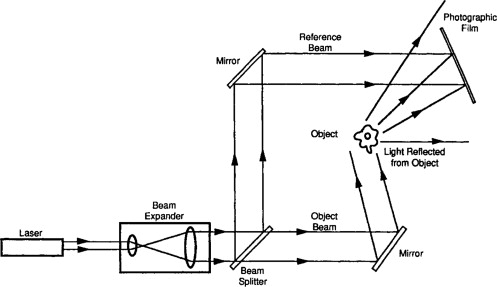
\includegraphics[width=0.9\linewidth]{figures/全息图的构建}
  \caption{全息图的构建光路}
\end{figure}

其中感光的器件可以用一些化学材料,也可以用光传感器。使用感光材料制作全息传感器的时候需要考虑材料对激光的敏感程度、材料对光强的响应是不是线性的,以及拍摄全息图的时候的噪声是否足够小。综合考虑这几种因素之后才能确保得到清晰度高的图像。

其次,全息装置的容错率是及其微小的,环境的微小变化,例如压强、温度,都会对精密的全息图造成影响,而一个微小的影响就足以让全息图没有办法复现。当然实验台要稳定,如果实验仪器发生了振动,那会造成更大的影响。

得到的全息图应当是交替变化的亮暗条纹,其中亮的地方表示参考光和测量光干涉相长,相位相同。暗的地方表示参考光和测量光相位相反,相互干涉抵消。因此通过拍摄全息图,把光的相位信息和强度信息合并成成为一个光的强度信息。

在用光路构建全息图的时候,有一个技巧就是在放置物体之前,先将光路仔细调节使得感光器件上形成干涉条纹,而且条纹越细得到的干涉图样就越好。我们在做实验的时候得到的这个结论。而且在实验中观察到放入物体后干涉条纹发生了弯曲。因此可能是图像的信息和干涉条纹的弯曲有关,条纹密集程度和图像分辨率正相关。

\subsection{再现全息图}

前面我们得到的全息图是来自物体的光和参考光叠加的光强分布。为了再现全息图我们需要想办法在已知参考光全部信息和参考光与来自物体的测量光叠加干涉后的光强信息的情况下,得到来自物体的测量光。

很显然,我们如果能在全息图中干涉后的光中减去参考光,就能得到来自物体的测量光。全息图再现的装置如下

\begin{figure}[H]
  \centering
  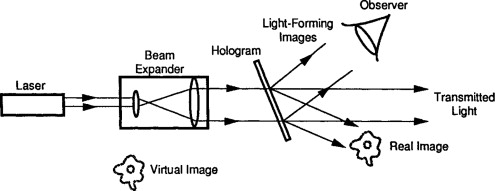
\includegraphics[width=0.9\linewidth]{figures/全息图的再现}
  \caption{全息图的再现光路}
\end{figure}

仔细与全息图的构建光路相比,可以发现:这个再现的光路和在全息图构建光路中遮挡住照射物体的光时的光路一样。只不过由于没有实际的物体,人眼看到的原来是实物的地方变为了虚物。

以上的全息是菲涅尔全息,菲涅尔全息需要被记录的物体和感光的器件之间距离比较近。基于菲涅尔全息的全息技术有很多变种,这是最基本的技术。所有基于菲涅尔全息的技术都是再现的时候用参考光照射全息图,并且都会在参考光的那侧生成虚像、在观察者的那一侧生成实像。

具体的原理涉及到傅立叶变换,根据傅立叶变换,这样的全息图生成的平面波是物体的傅立叶变换。

\subsection{全息图同普通图像相比较的优势的劣势}

全息摄影被称为“不需要透镜的摄影”,因为捕获的图像不是聚焦在一个胶卷上的图像(像照相机照相的时候,有一个镜头将远处的景象聚焦在胶卷上),全息图记录的是一个干涉图样。由于记录了光的相位信息,再现的时候生成的虚像就在原来的位置,因此观察者在不同的角度会观察到不同的像。

\begin{figure}[H]
  \centering
  \begin{subfigure}{0.96\linewidth}
    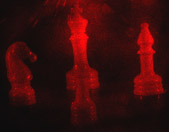
\includegraphics[width=\linewidth]{figures/全息拍摄中}
    \subcaption{在中央拍摄的全息图}
  \end{subfigure}
  \begin{subfigure}{0.48\linewidth}
    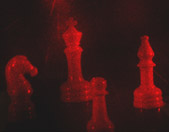
\includegraphics[width=\linewidth]{figures/全息拍摄左}
    \subcaption{在左边拍摄的全息图}
  \end{subfigure}
  \begin{subfigure}{0.48\linewidth}
    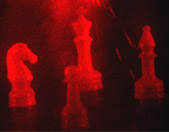
\includegraphics[width=\linewidth]{figures/全息拍摄右}
    \subcaption{在右边拍摄的全息图}
  \end{subfigure}
  \caption{同一张全息图在不同位置用摄像机拍摄的图像}
\end{figure}

上面展示了一张全息图在不同位置观测的图像,将摄像机分别放置于中间和左右两边,拍摄全息再现时的图像。可以看出三张图四个棋子的位置发生了相对变化,这表明全息记录的图像是三维的。
\section{全息技术的发展与应用}

\subsection{360度全息影响展示}

上面介绍的全息技术虽然是三维图像,但是观察者只能在固定的角度观看图像。现在比较前沿的技术是360度全息技术,其中比较成熟的是用四块透明的材质组成类似四面体的结构,参考光从下面照射上来,照亮四块透明的全息板,这样就使得360度都能观看图像。

\begin{figure}[H]
  \centering
  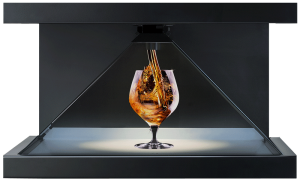
\includegraphics[width=0.9\linewidth]{figures/3D全息}
  \caption{一个3D全息展台,投影展示展品}
\end{figure}

当然也有不需要借助透明的全息板,直接把全息图投射到空气中的技术,也有在空气中掺杂其他成分之后把全息图投射到空气中的技术,只不过现在这些技术不够成熟。

\subsection{裸眼3D技术}

应用全息图的3D特性,可以开发裸眼3D技术。即不用借助任何眼镜之类的工具,只用人眼就能观看的3D图像。目前的3D电影之类的技术还停留在必须用眼镜的时代,即佩戴一副眼镜,眼镜的两个镜片是不同方向的偏振片,屏幕上为左眼和右眼分别播放了不同的偏振方向的图像,导致佩戴眼镜的人左右眼看到的图像不一样。这种3D解决方案不算真正的3D,因为左眼和右眼看到的都是二维图像,只是因为左右眼图像的差异模拟了视角差让人误以为是3D图像,实际上你更换观察者的位置图像不会改变。但是全息技术就跟这个有本质的区别,观看全息再现的图像时,观察者看的是一个虚像而不是一个照片。

\subsection{全息在AR教学方面的应用}

应用全息的技术,可以让用户看到不同的3D图像,因此可以更改全息投影仪投射的光,因而让用户看到的3D图像变换起来,起到直观的增强现实(Augmented reality)展示效果。

\end{multicols}

\begin{thebibliography}{99}  
\bibitem{ref1} Holography - Wikipedia, https://en.wikipedia.org/wiki/Holography
\bibitem{ref2} Holography - an overview, Science Direct, https://www.sciencedirect.com/topics/physics-and-astronomy/holography
\bibitem{ref3} Holographic Sensors: Three-Dimensional Analyte-Sensitive Nanostructures and Their Applications, https://pubs.acs.org/doi/10.1021/cr500116a
\bibitem{ref4} Holography, http://hyperphysics.phy-astr.gsu.edu/hbase/optmod/holog.html

\bibitem{ref5} 3D hologram - a short, simple explanation, https://magic-holo.com/en/what-is-a-3d-hologram/

\end{thebibliography}


\end{document}

%%% Local Variables:
%%% mode: latex
%%% TeX-master: t
%%% End:
